%!TEX program = xelatex
% 完整编译: xelatex -> biber/bibtex -> xelatex -> xelatex
\documentclass[lang=cn,a4paper,newtx,bibend=bibtex]{elegantpaper}

\title{Theoretical Questions of Chapter 3}
\author{张志心 \ 混合2106}

\date{\zhdate{2023/11/15}}

% \qedhere to make the square straight after

\usepackage{array}
\usepackage{tcolorbox}
\usepackage{tikz}
\usepackage{pgfplots}
\usepackage{float}

\newtcolorbox{prob}[1][]{
  colframe=gray,
  colback=white,
  boxrule=1.5pt, % 控制外边框线的宽度
  sharp corners, % 使用直角边框
  fonttitle=\bfseries,
  title=#1
}

\newcommand{\ccr}[1]{\makecell{{\color{#1}\rule{1cm}{1cm}}}}
\pgfplotsset{compat=1.17}

\addbibresource[location=local]{reference.bib}

\begin{document}

\maketitle



\begin{prob}[3.6.1-\textrm{I}.]
  Consider $s\in\mathbb{S}_3^2$ on $[0,2]$:
  \begin{equation*}
    s(x)=\begin{cases} p(x) & \text{if~} x\in[0,1],\\ (2-x)^3 & \text{if~} x\in[1,2].\end{cases}
  \end{equation*}
  Determine $p\in\mathbb{P}_3$ such that $s(0)=0$.
  Is $s(x)$ a natural cubic spline?
\end{prob}

\begin{solution}
设 $p(x) = ax^3 + bx^2 + cx$,根据 $\mathbb{S}_3^2$ 的条件,$p(x)$ 满足
$p(1) = 1, p'(1) = -3, p''(1) = 6$。

\begin{equation*}
  \begin{cases}
    a + b + c = 1 \\
    3a + 2b + c = -3 \\
    6a + 2b = 6
  \end{cases}
\end{equation*}
  解得,$(a, b, c) = (7, -18, 12)$,所以 $p(x) = 7x^3 - 18 x^2 + 12$。
  由于 $s''(0) = p''(0) = -36 \neq 0$,所以 $s(x)$ 不是自然三次样条函数。
\end{solution}

\begin{prob}[3.6.1-\textrm{II}.]
  Given $f_i=f(x_i)$ of some scalar function at points $a= x_1 < x_2 < \cdots < x_n = b$, we consider interpolating $f$ on $[a,b]$ with a quadratic spline $s\in\mathbb{S}_2^1$.
  \begin{enumerate}[(a)]
    \item Why is an additional condition needed to determine $s$ uniquely?
    \item Define $m_i=s'(x_i)$ and $p_i=s\big|_{[x_i,x_{i+1}]}$. Determine $p_i$ in terms of $f_i,f_{i+1}$ and $m_i$ for $i=1,2,...,n-1$.
    \item Suppose $m_1=f'(a)$ is given. Show how $m_2,m_3,...,m_{n-1}$ can be computed.
  \end{enumerate}
\end{prob}

\begin{solution} ~~%<br>

\begin{enumerate}[(a)]
  \item 一共需要求得 $n-1$ 个区间上的二次函数,共 $3(n-1)$ 个未知系数。定义 $p_i = s\big|_{[x_i, x_{i+1}]}$。
  
  已知 $p_{i}(x_i) = f_i, p_{i}(x_{i+1}) = f_{i+1},i = 1, \cdots, n-1$ 以及 $p_{i}'(x_{i+1}) = p_{i+1}'(x_{i+1}), i = 1, \cdots, n-2$。

  共有 $3n-4$ 个条件,因此要唯一确定 $s$ 还需要一个额外的条件。
  \item 根据条件 $p_i(x_i) = f_i, p_i(x_{i+1}) = f_{i+1}, p_i'(x_i) = m_i$。计算差商表如下:
  
  \begin{tabular}{c|ccc}
    &&& \\
    \hline
    \textbf{$x_i$} & $f_i$ & &  \\
    \textbf{$x_i$} & $f_i$ & $m_i$  &  \\
    \textbf{$x_{i+1}$} & $f_{i+1}$ & $\frac{f_{i+1} - f_i}{x_{i+1} - x_i}$ & $\frac{f_{i+1} - f_i - m_i(x_{i+1} - x_i)}{(x_{i+1} - x_i)^2}$ \\
  \end{tabular}
  所以 $p_i(x) = f_i + m_i(x - x_i) + \frac{f_{i+1} - f_i - m_i(x_{i+1} - x_i)}{(x_{i + 1} - x_i)^2}(x - x_i)^2 $。
  \item 由 (2),因为 $m_{i + 1} = p_i'(x_{i+1})$,则
  \[m_{i + 1} = p_i'(x_{i+1}) = m_i + \frac{2[f_{i + 1} - f_i - m_i(x_{i + 1} - x_i)]}{(x_{i + 1} - x_i)} = 2\frac{f_{i +1} - f_i}{x_{i + 1} - x_i} - m_i\]
  所以可以通过 $m_1, f_1, \cdots, f_{n}$ 递推地求出 $m_2, \cdots, m_n$。
\end{enumerate}
\end{solution}

\begin{prob}[3.6.1-\textrm{III}.]
  Let $s_1(x)=1+c(x+1)^3$ where $x\in[-1,0]$ and $c\in \mathbb{R}$. Determine $s_2(x)$ on $[0,1]$ such that
  
  \begin{equation*}
    s(x)=\begin{cases} s_1(x) & \text{if~} x\in[-1,0]\\ s_2(x) & \text{if~} x\in [0,1]\end{cases}
  \end{equation*}
  
  is a natural cubic spline on $[-1,1]$ with knots $-1,0,1$. How must $c$ be chosen if one wants $ s(1) = -1$?
\end{prob}

\begin{solution}
由 $s_1(0) = 1 + c,  s_1'(0) = 3c, s_1''(0) = 6c$ 得 $s_2(x) = 1 + c + 3cx + 6cx^2 + kx^3$,

由于是自然三次样条,所以 $s_2''(1) = 6k + 12c = 0$,

所以 $s_2(x) = 1+c+3cx+6cx^2-2cx^3$,

代入$s(1)=1+8c=-1$,得 $c = -\frac{1}{4}$。
\end{solution}

\begin{prob}[3.6.1-\textrm{IV}.]
  Consider $f(x)=\cos\left(\frac{\pi}{2}x\right)$ with $x\in[-1,1]$.
  \begin{enumerate}[(a)]
    \item Determine the natural cubic spline interpolant to $f$ on knots $-1,0,1$.
    \item As discussed in the class, natural cubic splines have the minimal total bending energy. Verify this by taking $g(x)$ be ($\mathrm{i}$) the quadratic polynomial that interpolates $f$ at $-1,0,1$, and ($\mathrm{ii}$) $f(x)$.
  \end{enumerate}
\end{prob}

\begin{solution}
\begin{enumerate}[(a)]
\item 根据条件 $s(-1) = 0, s(0) = 1, s(1) = 0, s''(-1) = s''(1) = 0$ 计算差商表如下:
\begin{tabular}{c|ccc}
&&&\\
\hline
-1 & 0 & & \\
0 & 1 & 1 & \\
1 & 0 & -1 & -1
\end{tabular}
由 $\frac12 s''(-1) + 2s''(0) + \frac12 s''(1) = 6f[-1, 0, 1] = -6$,所以 $s''(0) = -3$。所以
\begin{equation*}
\begin{aligned}
&s'(-1) = f[-1, 0] - \frac16 (s''(0) + 2s''(-1)) = \frac32 \\
&s'(0) = f[0, 1] - \frac16(s''(1) + 2s''(0)) = 0 \\
&s'''(-1) = \frac{s''(0) - s''(-1)}{0 - (-1)} = -3 \\
&s'''(0) = \frac{s''(1) - s''(0)}{1 - 0} = 3
\end{aligned}
\end{equation*}
计算得到
\[
  s(x) = \begin{cases}-\frac12 x^3 - \frac32 x^2 +1 & x\in [-1, 0]\\ \frac12 x^3 - \frac32 x^2 + 1 & x \in [0, 1]\end{cases}
\]
\item $s''(x) = \begin{cases} -3x - 3 & x\in [-1, 0] \\ 3x - 3 & x\in [0, 1]\end{cases}$,则
$\int_{-1}^1 \left[s''(x)\right]^2\mathrm{d}x = \int_{-1}^0 (-3x-3)^2 \mathrm{d}x + \int_0^1 (3x-3)^2\mathrm{d}x = 6$。
\begin{enumerate}[(i)]
\item $g(x) = (x + 1) - x(x + 1) = -x^2 + 1$, $g''(x) = -2$, 
\[\int_{-1}^1 \left[g''(x)\right]^2 \mathrm{d}x = 8 > 6\]
\item $f''(x) = \frac{-\pi^2}{4}\cos{(\frac{\pi}2x)}$, 
\[\int_{-1}^1 \left[f''(x)\right]^2\mathrm{d}x = \frac{\pi^4}{16}\int_{-1}^1 \cos^2(\frac{\pi}2x)\mathrm{d}x = \frac{\pi^4}{16} \approx 6.088 > 6\].
\end{enumerate}
\end{enumerate}
\end{solution}

\begin{prob}[3.6.1-\textrm{V}.]
  The quadratic B-spline $B_i^2(x)$.
  \begin{enumerate}[(a)]
    \item Derive the same explicit expression of $B_i^2(x)$ as that in the notes from the recursive definition of B-splines and the hat function.
    \item Verify that $\frac{\text{d}}{\text{d}x}B_i^2(x)$ is continuous at $t_i$ and $t_{i+1}$.
    \item Show that only one $x^*\in(t_{i-1},t_{i+1})$ satisfies $\frac{\text{d}}{\text{d}x}B_i^2(x^*)=0$. Express $x^*$ in terms of the knots within the interval of support.
    \item Consequently, show $B_i^2(x)\in[0,1)$.
    \item Plot $B_i^2(x)$ for $t_i=i$.
  \end{enumerate}
\end{prob}

\begin{solution}~~%<br>

  \begin{enumerate}[(a)]
    \item
    \begin{equation*}
      B_i^1(x)=\begin{cases}
        \frac{x-t_{i-1}}{t_i-t_{i-1}} & x\in(t_{i-1},t_i],\\
        \frac{t_{i+1}-x}{t_{i+1}-t_i} & x\in(t_i,t_{i+1}],\\
        0 & \text{others}.
      \end{cases}
      ~~~~~
      B_{i+1}^1(x)=\begin{cases}
        \frac{x-t_{i}}{t_{i+1}-t_{i}} & x\in(t_{i},t_{i+1}],\\
        \frac{t_{i+2}-x}{t_{i+2}-t_{i+1}} & x\in(t_{i+1},t_{i+2}],\\
        0 & \text{others}.
      \end{cases}
    \end{equation*}
    由于 $B_i^2(x)=\frac{x-t_{i-1}}{t_{i+1}-t_{i-1}}B_i^1(x)+\frac{t_{i+2}-x}{t_{i+2}-t_{i}}B_{i+1}^1(x)$,
    
    当 $x\in(t_{i-1},t_i]$ 时,
    \[
      B_i^2(x)=\frac{x-t_{i-1}}{t_{i+1}-t_{i-1}}\cdot \frac{x-t_{i-1}}{t_i-t_{i-1}} = \frac{(x-t_{i-1})^2}{(t_{i+1}-t_{i-1})(t_i-t_{i-1})};
    \]
    当 $x\in(t_{i},t_{i+1}]$ 时,
    \[
      B_i^2(x)=\frac{x-t_{i-1}}{t_{i+1}-t_{i-1}}\cdot \frac{t_{i+1}-x}{t_{i+1}-t_i} + \frac{t_{i+2}-x}{t_{i+2}-t_i}\cdot \frac{x - t_i}{t_{i+1}-t_i} = \frac{(x-t_{i-1})(t_{i+1}-x)}{(t_{i+1}-t_{i-1})(t_{i+1}-t_i)}+\frac{(t_{i+2}-x)(x-t_i)}{(t_{i+2}-t_{i})(t_{i+1}-t_{i})};
    \]
    当 $x\in(t_{i+1},t_{i+2}]$ 时,
    \[
      B_i^2(x) = \frac{t_{i+2}-x}{t_{i+2}-t_i}\cdot \frac{t_{i+2}-x}{t_{i+2}-t_{i+1}} = \frac{(t_{i+2}-x)^2}{(t_{i+2}-t_{i})(t_{i+2}-t_{i+1})}.
    \]
    对于其他情况,$B_i^2(x) = 0$。

    \item
    \[
      \frac{\mathrm{d}}{\mathrm{d}x} B_i^2(x) = \begin{cases}
        \frac{2(x-t_{i-1})}{(t_{i+1}-t_{i-1})(t_i-t_{i-1})} & x\in(t_{i-1},t_i]\\
        \frac{-2x+(t_{i+1}+t_{i-1})}{(t_{i+1}-t_{i-1})(t_{i+1}-t_i)}+\frac{-2x+(t_i+t_{i+2})}{(t_{i+2}-t_{i})(t_{i+1}-t_{i})} & x\in(t_i,t_{i+1}]\\
        \frac{-2(t_{i+2}-x)}{(t_{i+2}-t_{i})(t_{i+2}-t_{i+1})} & x\in(t_{i+1},t_{i+2}]\\
        0 & \text{others}.
      \end{cases}
    \]

    计算得到
    \begin{equation*}
    \begin{aligned}
      \frac{\mathrm{d}}{\mathrm{d}x}B_i^2(t_i)=\lim_{x\to t_i^{-}}\frac{\mathrm{d}}{\mathrm{d}x}B_i^2(x) &= \frac2{t_{i+1}-t_{i-1}} \\
      \lim_{x\to t_i^{+}}\frac{\mathrm{d}}{\mathrm{d}x}B_i^2(x) &= \frac{-2t_i+(t_{i+1}+t_{i-1})}{(t_{i+1}-t_{i-1})(t_{i+1}-t_i)}+\frac{-2t_i+(t_i+t_{i+2})}{(t_{i+2}-t_{i})(t_{i+1}-t_{i})}\\ 
      &= \frac{-2t_i(t_{i+2}-t_i+t_{i+1}-t_{i-1})+(t_{i+1}+t_{i-1})(t_{i+2}-t_i)+(t_i+t_{i+2})(t_{i+1}-t_{i-1})}{(t_{i+1}-t_{i-1})(t_{i+1}t_{i+2}+t_i^2-t_i(t_{i+1}+t_{i+2}))} \\
      &= \frac{-2t_it_{i+2}+2t_i^2-2t_it_{i+1}+2t_it_{i-1}+2t_{i+1}t_{i+2}-2t_it_{i-1}}{(t_{i+1}-t_{i-1})(t_{i+1}t_{i+1}+t_i^2-t_it_{i+1}-t_it_{i+2})} \\
      &= \frac{2}{t_{i+1} - t_{i-1}} = \lim_{x\to t_i}\frac{\mathrm{d}}{\mathrm{d}x}B_i^2(x) = \frac{\mathrm{d}}{\mathrm{d}x}B_i^2(t_i)
    \end{aligned}
    \end{equation*}
    \begin{equation*}
      \begin{aligned}
        \frac{\mathrm{d}}{\mathrm{d}x}B_i^2(t_{i+1})=\lim_{x\to t_{i+1}^{-}}\frac{\mathrm{d}}{\mathrm{d}x}B_i^2(x) &= \frac{-2}{t_{i+2}-t_i} \\
        \lim_{x\to t_{i+1}^{+}}\frac{\mathrm{d}}{\mathrm{d}x}B_i^2(x) &= \frac{-2(t_{i+2}-t_{i+1})}{(t_{i+2}-t_{i})(t_{i+2}-t_{i+1})}\\
        &= \frac{-2}{t_{i+2}-t_i} = \lim_{x\to t_{i+1}}\frac{\mathrm{d}}{\mathrm{d}x}B_i^2(t_{i+1}) = \frac{\mathrm{d}}{\mathrm{d}x}B_i^2(t_{i+1})
      \end{aligned}
      \end{equation*}
    所以 $\frac{\mathrm{d}}{\mathrm{d}x}B_i^2(x)$ 在 $t_i$ 和 $t_{i+1}$ 处连续。

    \item 因为 
    $\lim_{x\to t_{i-1}^+}\frac{\mathrm{d}}{\mathrm{d}x}B_i^2(x)=\frac{\mathrm{d}}{\mathrm{d}x}B_i^2(t_{i+2}) = 0,\frac{\mathrm{d}}{\mathrm{d}x}B_i^2(t_i)=\frac{2}{t_{i+1}-t_{i-1}}>0,\lim_{x\to t_{i+1}}\frac{\mathrm{d}}{\mathrm{d}x}B_i^2(x) = \frac{-2}{t_{i+2}-t_i} < 0$,
    $B_i^2(x)$ 是线性函数,所以 $(t_{i_1}, t_i)$ 和 $(t_{i+1}, t_{i+2})$ 中不存在零点。

    当 $x\in [t_{i}, t_{i+1}]$ 时,
    \[
      \frac{-2x^*+(t_{i+1}+t_{i-1})}{(t_{i+1}-t_{i-1})(t_{i+1}-t_i)}+\frac{-2x^*+(t_{i+2}+t_i)}{(t_{i+2}-t_i)(t_{i+1}-t_i)}=0 \Rightarrow x^*=\frac{t_{i+1}t_{i+2}-t_{i-1}t_i}{t_{i+2}+t_{i+1}-t_i-t_{i-1}}
    \]
    \item 根据 (c) 可以得到,
    \begin{equation*}
    % \begin{aligned}
      \begin{cases}
      \frac{\mathrm{d}}{\mathrm{d}x}B_i^2(x)>0, ~~~~ x\in(t_{i-1},x^*)\\
      \frac{\mathrm{d}}{\mathrm{d}x}B_i^2(x)<0, ~~~~ x\in(x^*,t_{i+2})
      \end{cases}
    % \end{aligned}
    \end{equation*}
    \begin{equation*}
    \begin{aligned}
    B_i^2(x^*) &= \frac{-2x^*+(t_{i+1}+t_{i-1})}{(t_{i+1}-t_{i-1})(t_{i+1}-t_i)}+\frac{-2x^*+(t_i+t_{i+2})}{(t_{i+2}-t_{i})(t_{i+1}-t_{i})}\\
    &= \frac{(t_{i+1}-t_{i-1})(t_{i+2}-t_{i-1})(t_{i+1}-t_{i-1})(t_{i+1}-t_i)}{(t_{i+1}-t_{i-1})(t_{i+1}-t_i)(t_{i+2}+t_{i+1}-t_i-t_{i-1})^2} + 
    \frac{(t_{i+2}-t_{i-1})(t_{i+2}-t_{i})(t_{i+1}-t_{i})(t_{i+2}-t_i)}{(t_{i+2}-t_{i})(t_{i+1}-t_i)(t_{i+2}+t_{i+1}-t_i-t_{i-1})^2} \\
    &= \frac{(t_{i+2}-t_{i-1})(t_{i+2}+t_{i+1}-t_i-t_{i-1})}{(t_{i+2}+t_{i+1}-t_i-t_{i-1})^2} \\
    &= \frac{t_{i+2}-t_{i-1}}{t_{i+2}+t_{i+1}-t_i-t_{i-1}} < 1
    \end{aligned}
    \end{equation*}
    所以 $B_i^2(x) \in [0, 1)$。
    \item
    \begin{equation*}
      B_i^2(x) = \begin{cases}
        \frac{(x-i+1)^2}{2} & x\in [i-1, i] \\
        -x^2+(2i+1)x-i^2-i+\frac12 & x\in [i, i+1] \\
        \frac{(i+2-x)^2}{2} & x\in [i+1, i+2]
      \end{cases}
    \end{equation*}

    \begin{center}
    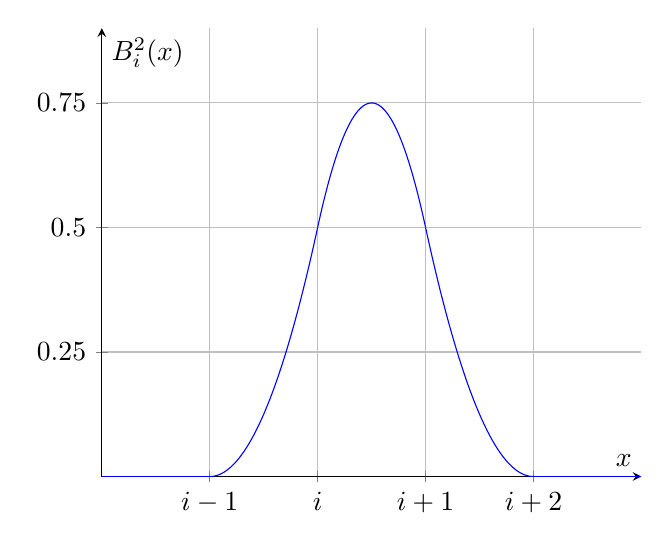
\begin{tikzpicture}
      \begin{axis}[
        xlabel=$x$,
        ylabel=$B_i^2(x)$,
        axis lines=middle,
        legend pos=outer north east,
        grid=both,
        % minor tick num=1,
        xtick={1.5,2.5,3.5,4.5},
        xticklabels={$i-1$, $i$, $i+1$, $i+2$},
        ytick={0.25,0.5,0.75,1},
        yticklabels={0.25,0.5,0.75,1},
        ymax=0.90
      ]
        \foreach \i in {2.5} {
            \addplot[domain=\i-2:\i-1, blue, samples=100] {0};
            \addplot[domain=\i-1:\i, blue, samples=100] {((x-\i+1)^2)/2};
            \addplot[domain=\i:\i+1, blue, samples=100] {(-x^2 + (2*\i + 1)*x - \i^2 - \i + 1/2)};
            \addplot[domain=\i+1:\i+2, blue, samples=100] {((\i+2-x)^2)/2};
            \addplot[domain=\i+2:\i+3, blue, samples=100] {0};
        }
      \end{axis}
    \end{tikzpicture}
  \end{center}

  \end{enumerate}
\end{solution}

\newpage

\begin{prob}[3.6.1-\textrm{VI}.]
  Verify Theorem 3.32 algebraically for the case of $n=2$, i.e.
  \begin{equation*}
    (t_{i+2}-t_{i-1})[t_{i-1},t_i,t_{i+1},t_{i+2}](t-x)_+^2=B_i^2(x).
  \end{equation*}
\end{prob}

\begin{solution}
当 $x\in (t_{i-1}, t_i]$ 时,
\begin{equation*}
\begin{aligned}
&[t_{i-1},t_i,t_{i+1},t_{i+2}](t-x)_+^2\\
=&\frac{
  \frac{
    \frac{(t_{i+2}-t_{i+1})(t_{i+2}-t_{i+1}-2x)}{t_{i+2}-t_{i+1}}
    -\frac{(t_{i+1}-t_{i})(t_{i+1}-t_{i}-2x)}{t_{i+1}-t_{i}}
  }{t_{i+2}-t_i}
  -
  \frac{
    \frac{(t_{i+1}-t_{i})(t_{i+1}-t_{i}-2x)}{t_{i+1}-t_{i}}
    -\frac{(t_i-x)^2}{t_{i}-t_{i-1}}
  }{t_{i+2}-t_i}
}{t_{i+2}-t_{i-1}} \\
=& \frac{1-\frac{t_{i+1+t_i-2x-\frac{(t_i-x)^2}{t_{i}-t_{i-1}}}}{t_{i+1}-t_{i-1}}}{t_{i+2}-t_{i-1}} 
=\frac{(2x-t_{i-1}-t_i)(t_i-t_{i-1})-(t_i-x)^2}{(t_{i+2}-t_{i-1})(t_{i+1}-t_{i-1})(t_i-t_{i-1})} \\
=& \frac{(x-t_{i-1})^2}{(t_{i+1}-t_{i-1})(t_i-t_{i-1})}\cdot \frac{1}{t_{i+2}-t_{i-1}} = \frac{B_i^2(x)}{t_{i+2}-t_{i-1}}
\end{aligned}
\end{equation*}

当 $x\in (t_{i}, t_{i+1}]$ 时,

\begin{equation*}
  \begin{aligned}
  &[t_{i-1},t_i,t_{i+1},t_{i+2}](t-x)_+^2\\
  =&\frac{
    \frac{
      \frac{(t_{i+2}-t_{i+1})(t_{i+2}-t_{i+1}-2x)}{t_{i+2}-t_{i+1}}
      -\frac{(t_{i+1}-x)^2}{t_{i+1}-t_{i}}
    }{t_{i+2}-t_i}
  }{t_{i+2}-t_{i-1}} 
  =\frac{\frac{-x^2+2t_ix-t_it_{i+1}-t_it_{i+2}+t_{i+1}t_{i+2}}{(t_{i+2}-t_i)(t_{i+1}-t_i)}-\frac{(t_{i+1}-x)^2}{(t_{i+1}-t_i)(t_{i+1}-t_{i-1})}}{t_{i+2}-t_{i-1}} \\
  =& \left[\frac{(x-t_{i-1})(t_{i+1}-x)}{(t_{i+1}-t_{i-1})(t_{i+1}-t_i)}+\frac{(t_{i+2}-x)(x-t_i)}{(t_{i+2}-t_{i})(t_{i+1}-t_{i})}\right] \cdot \frac{1}{t_{i+2}-t_{i-1}} = \frac{B_i^2(x)}{t_{i+2}-t_{i-1}}
  \end{aligned}
  \end{equation*}

当 $x\in (t_{i+1}, t_{i+2}]$ 时,
\begin{equation*}
  \begin{aligned}
    &[t_{i-1},t_i,t_{i+1},t_{i+2}](t-x)_+^2\\
    =&\frac{(t_{i+2}-x)^2}{(t_{i+2}-t_{i+1})(t_{i+2}-t_i)(t_{i+2}-t_{i-1})} \\
    =& \frac{(t_{i+2}-x)^2}{(t_{i+2}-t_{i})(t_{i+2}-t_{i+1})}\cdot \frac{1}{t_{i+2}-t_{i-1}} = \frac{B_i^2(x)}{t_{i+2}-t_{i-1}}
  \end{aligned}
\end{equation*}

当 $x\in (-\infty, t_{i-1}]$ 时,$[t_{i-1},t_i,t_{i+1},t_{i+2}](t-x)_+^2 = \frac{1-1}{t_{i+2}-t_{i-1}} = 0 = \frac{B_i^2(x)}{t_{i+2}-t_{i-1}}$.

当 $x\in (t_{i+2}, -\infty)$ 时 $[t_{i-1},t_i,t_{i+1},t_{i+2}](t-x)_+^2 = 0 = \frac{B_i^2(x)}{t_{i+2}-t_{i-1}}$.

所以 $(t_{i+2}-t_{i-1})[t_{i-1},t_i,t_{i+1},t_{i+2}](t-x)_+^2=B_i^2(x)$。
\end{solution}

\begin{prob}[3.6.1-\textrm{VII}.]
  Scaled integral of B-splines.

  Deduce from the Theorem on deriviates of B-splines that the 
  scaled integral of a B-spline $B_i^n(x)$ over its support is 
  independent of its index $i$ even if the spacing of the knots is not uniform.

\end{prob}

\begin{proof}
由 
\[
\frac{\mathrm{d}}{\mathrm{d}x} B_i^{n+1}(x) = \frac{(n+1)B_i^n(x)}{t_{i+n}-t_{i-1}}-\frac{(n+1)B_{i+1}^n(x)}{t_{i+n+1}-t_i}
\]
\begin{equation*}
\begin{aligned}
\int_{t_{i-1}}^{t_{i+n}} B_i^n(x)\mathrm{d}x &= \frac{t_{i+n}-t_{i-1}}{n+1} \left(B_i^{n+1}(t_{i+n})-B_i^{n+1}(t_{i-1})+\frac{n+1}{t_{i+n+1}-t_i}\int_{t_{i-1}}^{t_{i+n}}B_{i+1}^n(x)\mathrm{d}x \right) \\
&= \frac{t_{i+n}-t_{i-1}}{n+1}\left(B_i^{n+1}(t_{i+n})-B_i^{n+1}(t_{i-1})\right) \\
&~~~~+\frac{t_{i+n}-t_{i-1}}{t_{i+n+1}-t_i}\cdot \frac{t_{i+n+1}-t_i}{n+1} \left(B_{i+1}^{n+1}(t_{i+n})-B_{i+2}^{n+1}(t_{i-1})+\frac{n+1}{t_{i+n+2}-t_{i+1}}\int_{t_{i-1}}^{t_{i+n}}B_{i+2}^n(x)\mathrm{d}x\right) \\
&= \frac{t_{i+n}-t_{i-1}}{n+1}\left(B_i^{n+1}(t_{i+n})+B_{i+1}^{n+1}(t_{i+n})+\frac{n+1}{t_{i+n+2}-t_{i+1}}\int_{t_{i-1}}^{t_{i+n}} B_{i+2}^n(x)\mathrm{d}x \right) \\
&= \cdots \\
&= \frac{t_{i+n}-t_{i-1}}{n+1}\left(B_i^{n+1}(t_{i+n})+B_{i+1}^{n+1}(t_{i+n})+\cdots+B_{i+n}^{n+1}(t_{i+n})\right)+\frac{n+1}{t_{i+2n+1}-t_{i+n}}\int_{t_{i-1}}^{t_{i+n}} B_{i+n+1}^n(x)\mathrm{d}x \\
&= \frac{t_{i+n}-t_{i-1}}{n+1}
\end{aligned}
\end{equation*}
所以 $\frac{1}{t_{i+n}-t_{i-1}}\int_{t_{i-1}}^{t_{i+n}} B_i^n(x)\mathrm{d}x = \frac1{n+1}$ 与 $i$ 无关。
\end{proof}

\begin{prob}[3.6.1-\textrm{VIII}.]
  Symmetric Polynomials.

  We have a theorem on expressing complete symmetric polynomials as divided difference of monomials.
  \begin{enumerate}[(a)]
    \item Verify this theorem for $m=4$ and $n=2$ by working out the table of divided difference and comparing the result to the definition of complete symmetric polynomials.
    \item Prove this theorem by the lemma on the recursive relation on complete symmetric polynomials.
  \end{enumerate}
\end{prob}

\begin{proof}~~%<br>

\begin{enumerate}[(a)]
\item $x^4$ 在 $x_i, x_{i+1}, x_{i+2}$ 的差商表计算如下:

\begin{center}
\begin{tabular}{l|lll}
  &&&\\
  \hline
  $x_i$     & $x_i^4$     &                                          &                                                                                                 \\
  $x_{i+1}$ & $x_{i+1}^4$ & $(x_{i+1}^2+x_{i}^2)(x_{i+1}+x_{i})$     &                                                                                                 \\
  $x_{i+2}$ & $x_{i+2}^4$ & $(x_{i+2}^2+x_{i+1}^2)(x_{i+2}+x_{i+1})$ & $\frac{(x_{i+2}^2+x_{i+1}^2)(x_{i+2}+x_{i+1})-(x_{i+1}^2+x_{i}^2)(x_{i+1}+x_{i})}{x_{i+2}-x_i}$
\end{tabular}\end{center}

\begin{align*}
[x_i, x_{i+1}, x_{i+2}] x^4  &= \frac{(x_{i+2}^3+x_{i+2}^2x_{i+1}+x_{i+2}x_{i+1}^2+x_{i+1}^3)-(x_{i+1}^3+x_{i+1}^2x_i+x_{i+1}x_i^2+x_i^3)}{x_{i+2}-x_i} \\
&= x_{i+2}^2 + x_{i+2}x_i + x_i^2 + x_{i+1}x_{i+2} + x_{i+1}x_i + x_{i+1}^2 = \tau_2(x_i, x_{i+1}, x_{i+2})
\end{align*}

\item $n = 0$ 时,$\tau_m(x_i) = [x_i]x^m = x_i^m$,设结论对 $n(<m)$ 时成立,
则 \[\tau_{m-n} = [x_i, \cdots, x_{i+n}]x^m, \tau_m(x_{i+1}, \cdots, x_{i+n+1}) = [x_{i+1}, \cdots, x_{i+n+1}]x^m,\]
\begin{align*}
&  \tau_{m-n-1}(x_i, \cdots, x_{i+n+1}) = \frac{\tau_{m-n}(x_{i+1},\cdots,x_{i+n+1}) - \tau_{m-n}(x_i, \cdots, x_{i+n})}{x_{i+n+1}-x_{i+n}} = [x_i, \cdots, x_{i+n+1}]x^m \\
\Leftrightarrow& (x_{i+n+1}-x_i)\tau_{m-n-1}(x_i,\cdots, x_{i+n+1}) = \tau_{m-n}(x_{i+1}, \cdots, x_{i+n+1}) - \tau_{m-n}(x_i, \cdots, x_{i+n}) \\
\Leftrightarrow& \tau_{m-n}(x_i, \cdots, x_{i+m}) + x_{i+n+1}\tau_{m-n-1}(x_i, \cdots, x_{i+n+1}) = \tau_{m-n}(x_i, \cdots, x_{i+n+1}) + x_i\tau_{m-n-1}(x_i, \cdots, x_{i+n+1})
\end{align*}

因为 $\text{LHS} = \text{RHS} = \tau_{m-n}(x_i, \cdots, x_{i+n+1})$,所以 $\tau_{m-n-1}(x_i,\cdots, x_{i+n+1}) = [x_i, \cdots, x_{i+n+1}]x^m$ 成立。

根据归纳假设,
\[\forall m\in \mathbb{N}^+, \forall i \in \mathbb{N}, \forall n = 0,1,\cdots, m, \tau_{m-n}(x_i, \cdots, x_{i+n}) = [x_i, \cdots, x_{i+n}]x^m.\]

\end{enumerate}
\end{proof}

\end{document}